This section is a tour through Gaussian and \textit{almost-Gaussian} quantum receivers which are used to discriminate between two coherent states $\ket{\pm \alpha}$ of equal energy and opposite phase. Note that such encoding is known in the literature as Binary Phase-Shifted Key (BPSK) coherent state discrimination, since the (classical) information is encoded into the phase of the coherent states. For simplicity, we assume that the sender and receiver have a shared reference frame, so that we can take the states to be real, \textit{e.g.} $\alpha\in\mathbb{R}$, without loss of generality, as shown in Fig.~\ref{fig:300coh}.
\begin{figure}[t!]
    \centering
    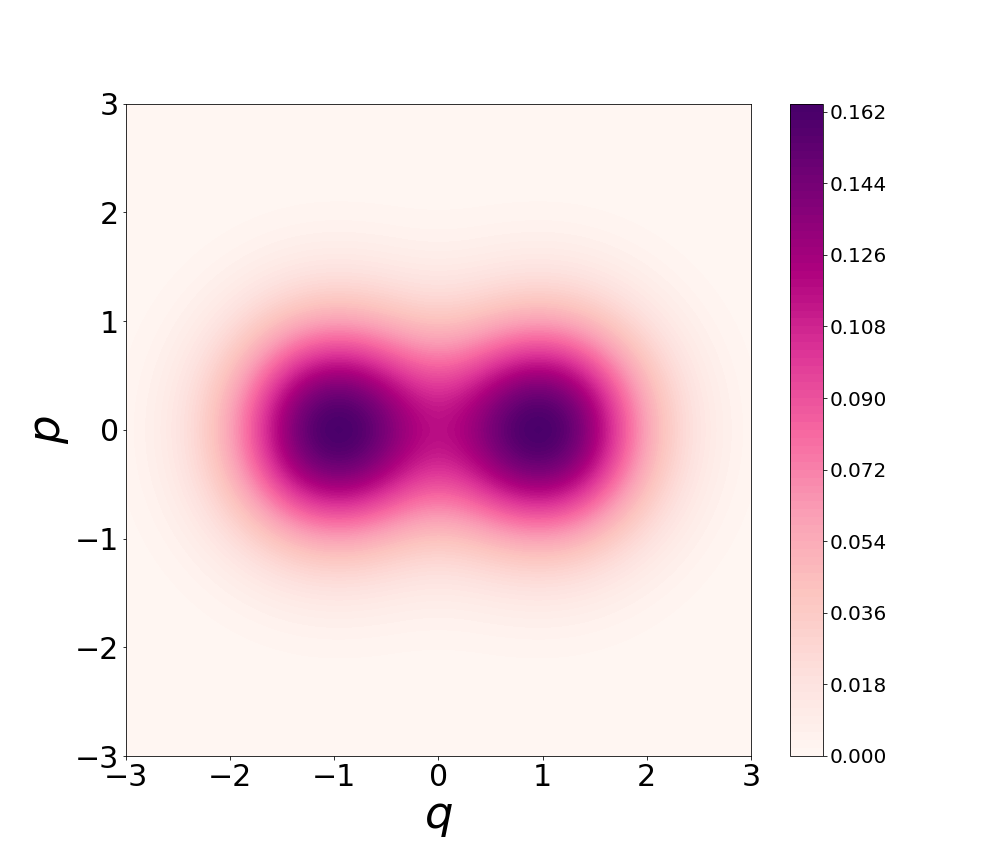
\includegraphics[width=0.8\textwidth]{Figures/some_wigners/bpshcoh.png}
    \caption{We show the Wigner function for the two candidate states $\ket{\alpha_k}, \; k=0,1$, which are Gaussian distribution functions. We restrict to real amplitudes, since in the binary case one can always rotate the frame (assuming we know the direction to do so).}
    \label{fig:300coh}
\end{figure}
The term quantum receiver stands for a quantum measurement that decodes the information carried out on a quantum state that was sent through a quantum channel. In this Section we will restrict to the case where the signals are not altered by neither the presence of a quantum channel (\textit{e.g.} we consider the noiseless channel) nor by noise due to malfunctioning devices: we will deal with such scenarios in Sec.~\ref{ssec:rlcoh_noise}.

As discussed in Sec.~\ref{ssec:1_cv_measurements}, operations in continuous-variable systems can be classified as either Gaussian or non-Gaussian. Generally, the Gaussian ones are considered \textit{feasible} in quantum optics laboratories. As such, they include linear operations (\textit{i.e.} displacing, phase-shifting, squeezing and mixing signals by beam-splitters), Gaussian POVMs (\textit{e.g.} homodyne and heterodyne measurements) and laser-beams. In particular, we observed in Sec.~\ref{ssec:intro_cv_phase} that coherent states are Gaussian states (\textit{e.g.} their Wigner function is a Gaussian distribution in phase-space), are obtained by displacing the vacuum state $\ket{\alpha} = \weyl{\alpha}\ket{0}$ and describe laser states.

This Section is structured as follows. We will comment on BPSK Gaussian receivers in Sec.~\ref{ssec:1_gaussian_receivers}. We then introduce some non-gaussianity through photon-detection measurements in Sec.~\ref{ssec:rlcoh_kennedyreceiver}, where we study the performance of the so-called \textit{Kennedy} receiver. Then, we will introduce the Dolinar receiver in Sec.~\ref{ssec:rlcoh_dolinarreceiver}, and explain its sequential logic throughout the section.
%Finally, we will pose the problem of calibrating Dolinar-like receivers as a reinforcement-learning one in Sec.~\ref{ssec:rlcoh_dolinar_2_RL}.
